\documentclass{article}\usepackage[]{graphicx}\usepackage[]{color}
%% maxwidth is the original width if it is less than linewidth
%% otherwise use linewidth (to make sure the graphics do not exceed the margin)
\makeatletter
\def\maxwidth{ %
  \ifdim\Gin@nat@width>\linewidth
    \linewidth
  \else
    \Gin@nat@width
  \fi
}
\makeatother

\definecolor{fgcolor}{rgb}{0.345, 0.345, 0.345}
\newcommand{\hlnum}[1]{\textcolor[rgb]{0.686,0.059,0.569}{#1}}%
\newcommand{\hlstr}[1]{\textcolor[rgb]{0.192,0.494,0.8}{#1}}%
\newcommand{\hlcom}[1]{\textcolor[rgb]{0.678,0.584,0.686}{\textit{#1}}}%
\newcommand{\hlopt}[1]{\textcolor[rgb]{0,0,0}{#1}}%
\newcommand{\hlstd}[1]{\textcolor[rgb]{0.345,0.345,0.345}{#1}}%
\newcommand{\hlkwa}[1]{\textcolor[rgb]{0.161,0.373,0.58}{\textbf{#1}}}%
\newcommand{\hlkwb}[1]{\textcolor[rgb]{0.69,0.353,0.396}{#1}}%
\newcommand{\hlkwc}[1]{\textcolor[rgb]{0.333,0.667,0.333}{#1}}%
\newcommand{\hlkwd}[1]{\textcolor[rgb]{0.737,0.353,0.396}{\textbf{#1}}}%

\usepackage{framed}
\makeatletter
\newenvironment{kframe}{%
 \def\at@end@of@kframe{}%
 \ifinner\ifhmode%
  \def\at@end@of@kframe{\end{minipage}}%
  \begin{minipage}{\columnwidth}%
 \fi\fi%
 \def\FrameCommand##1{\hskip\@totalleftmargin \hskip-\fboxsep
 \colorbox{shadecolor}{##1}\hskip-\fboxsep
     % There is no \\@totalrightmargin, so:
     \hskip-\linewidth \hskip-\@totalleftmargin \hskip\columnwidth}%
 \MakeFramed {\advance\hsize-\width
   \@totalleftmargin\z@ \linewidth\hsize
   \@setminipage}}%
 {\par\unskip\endMakeFramed%
 \at@end@of@kframe}
\makeatother

\definecolor{shadecolor}{rgb}{.97, .97, .97}
\definecolor{messagecolor}{rgb}{0, 0, 0}
\definecolor{warningcolor}{rgb}{1, 0, 1}
\definecolor{errorcolor}{rgb}{1, 0, 0}
\newenvironment{knitrout}{}{} % an empty environment to be redefined in TeX

\usepackage{alltt}
\usepackage[sc]{mathpazo}
\usepackage[T1]{fontenc}
\usepackage{geometry}
\usepackage[utf8]{inputenc}
\geometry{verbose,tmargin=2.5cm,bmargin=2.5cm,lmargin=2.5cm,rmargin=2.5cm}
\setcounter{secnumdepth}{2}
\setcounter{tocdepth}{2}
\usepackage{url}
\usepackage[unicode=true,pdfusetitle,
 bookmarks=true,bookmarksnumbered=true,bookmarksopen=true,bookmarksopenlevel=2,
 breaklinks=false,pdfborder={0 0 1},backref=false,colorlinks=false]
 {hyperref}
\hypersetup{
 pdfstartview={XYZ null null 1}}
\IfFileExists{upquote.sty}{\usepackage{upquote}}{}
\begin{document}



\title{Knitr Motores de lenguaje / Language Engines - Programación de aplicaciones para Internet y la Nube.}
\author{Andres Julian Moreno M. Cód. 20152195015}
\maketitle

El presente documento dinámico es generado para  el informe de programación literaria para informes de experimentos computacionales en la nube.\\

Es una herramienta la cual tiene por objetivo la generación de documentos dinámicos, esta herramienta funciona en el lenguaje R, y permite trabajar desde la interfaz Rstudio. Permitiendo integrar las funcionalidades de R en documentos de tipo científico y académicos LATEX, Markdown y también en documentos o publicaciones sobre HTML, a través de la programación literaria busca fortalecer la reproducibilidad de la investigación.\\

Knitr permite integrar R con otros lenguajes de programación como $python, Perl, C, C++, shell, Awk,\\ SAS, Scala, Haskell, Graphviz, TikZ y Coffeescript$ en un unico documento dinámico.\\

\subsubsection*{Por ejemplo vamos a ejecutar un trozo de R, sobre este documento dinámico de tipo R Markdown}
\begin{knitrout}
\definecolor{shadecolor}{rgb}{0.969, 0.969, 0.969}\color{fgcolor}\begin{kframe}
\begin{alltt}
\hlkwd{library}\hlstd{(knitr)}
\hlkwd{set.seed}\hlstd{(}\hlnum{1234}\hlstd{)}
\hlkwd{rnorm}\hlstd{(}\hlnum{5}\hlstd{)}
\end{alltt}
\begin{verbatim}
## [1] -1.2070657  0.2774292  1.0844412 -2.3456977  0.4291247
\end{verbatim}
\end{kframe}
\end{knitrout}

\subsubsection*{Con el siguiente comando observamos cuales son todos los lenguajes soportados por Knitr:} 
\begin{knitrout}
\definecolor{shadecolor}{rgb}{0.969, 0.969, 0.969}\color{fgcolor}\begin{kframe}
\begin{alltt}
\hlkwd{names}\hlstd{(knit_engines}\hlopt{$}\hlkwd{get}\hlstd{())}
\end{alltt}
\begin{verbatim}
##  [1] "awk"       "bash"      "coffee"    "gawk"      "groovy"    "haskell"   "lein"     
##  [8] "mysql"     "node"      "perl"      "psql"      "python"    "Rscript"   "ruby"     
## [15] "sas"       "scala"     "sed"       "sh"        "stata"     "zsh"       "highlight"
## [22] "Rcpp"      "tikz"      "dot"       "c"         "fortran"   "asy"       "cat"      
## [29] "asis"      "stan"      "block"
\end{verbatim}
\end{kframe}
\end{knitrout}

\subsubsection*{Ahora un Ejemplo de R un poco complejo incluyendo un par de gráficas, integrando el paquete de graficos para R ggplot2}
\begin{knitrout}
\definecolor{shadecolor}{rgb}{0.969, 0.969, 0.969}\color{fgcolor}\begin{kframe}
\begin{alltt}
\hlcom{## tomado de http://yihui.name/knitr/}
\hlstd{fit} \hlkwb{<-} \hlkwd{lm}\hlstd{(dist} \hlopt{~} \hlstd{speed,} \hlkwc{data} \hlstd{= cars)}
\hlkwd{par}\hlstd{(}\hlkwc{mar} \hlstd{=} \hlkwd{c}\hlstd{(}\hlnum{4}\hlstd{,} \hlnum{4}\hlstd{,} \hlnum{1}\hlstd{,} \hlnum{0.1}\hlstd{),} \hlkwc{mgp} \hlstd{=} \hlkwd{c}\hlstd{(}\hlnum{2}\hlstd{,} \hlnum{1}\hlstd{,} \hlnum{0}\hlstd{))}
\hlkwd{with}\hlstd{(cars,} \hlkwd{plot}\hlstd{(speed, dist,} \hlkwc{panel.last} \hlstd{=} \hlkwd{abline}\hlstd{(fit)))}
\hlkwd{text}\hlstd{(}\hlnum{10}\hlstd{,} \hlnum{100}\hlstd{,} \hlstr{"$Y = \textbackslash{}\textbackslash{}beta_0 + \textbackslash{}\textbackslash{}beta_1x + \textbackslash{}\textbackslash{}epsilon$"}\hlstd{)}
\hlkwd{library}\hlstd{(ggplot2)}
\hlkwd{qplot}\hlstd{(speed, dist,} \hlkwc{data} \hlstd{= cars)} \hlopt{+} \hlkwd{geom_smooth}\hlstd{()}
\end{alltt}
\end{kframe}

{\centering 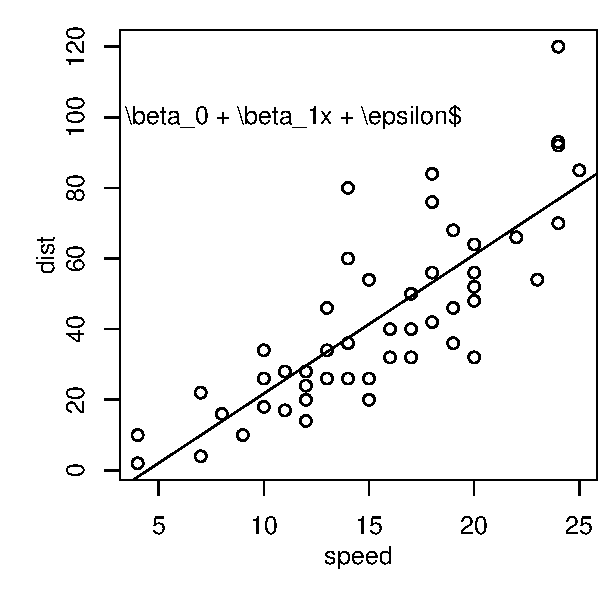
\includegraphics[width=.4\linewidth]{figure/minimal-r2-1} 
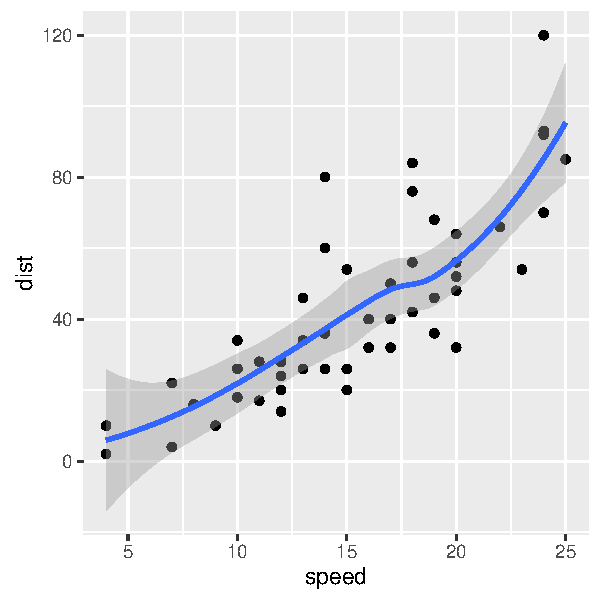
\includegraphics[width=.4\linewidth]{figure/minimal-r2-2} 

}



\end{knitrout}

\subsection*{Soporte}

Como los $chunk hooks$ (trozos de código), los motores o lenguajes están soportados por $Knitr$ y $R$.\\

Las funciones chunk se encargan de ejecutar el chunk (trozo de código) en el lenguaje determinado por el usuario y ejecutar el código en R, obteniendo resultados y mostrando su salida, para la mayoría de los casos, el código se comunica con los programas externos mediante la funciona del sistema, $system()$.\\

\subsection*{Como Funciona Knitr}

Todos los lenguajes que soporta Knitr son guardados en la función $knit_engines$, la cual cuenta con métodos $get()$ y $set()$, como la ejecución de funciones chunk hooks y chunk options, entonces si por ejemplo queremos generar un documento en Python se debe seleccionar la función `engine` y asignarle la opción de python, como por ejemplo $engine='python'$ o $engine='awk'$ si queremos ejecutar otro lenguaje. El objeto $knit_engines$ almacena una serie de funciones con nombre del lenguaje soportado.\\

\section*{Ejemplo en $Python$}

A continuación se muestran varios ejemplos de programas sencillos hechos en $Python$ y ejecutados en $R$, gracias a $Knitr$ y los $chunk engine$.

\subsubsection*{Programa 1: Mostrar numeros Naturales}
\begin{knitrout}
\definecolor{shadecolor}{rgb}{0.969, 0.969, 0.969}\color{fgcolor}\begin{kframe}
\begin{alltt}
n = 1
while n <= 30: 
    print n,
## Imprime los primeros 30 numeros naturales
    n += 1
\end{alltt}

\begin{verbatim}
## 1 2 3 4 5 6 7 8 9 10 11 12 13 14 15 16 17 18 19 20 21 22 23 24 25 26 27 28 29 30
\end{verbatim}
\end{kframe}
\end{knitrout}

\subsubsection*{Programa 2: Sumas}
\begin{knitrout}
\definecolor{shadecolor}{rgb}{0.969, 0.969, 0.969}\color{fgcolor}\begin{kframe}
\begin{alltt}
## Imprime la suma de 1+2+3+4+....+50
h = range(1, 51)
print sum(h)
\end{alltt}

\begin{verbatim}
## 1275
\end{verbatim}
\end{kframe}
\end{knitrout}

\subsubsection*{Programa 3: Hola Mundo}
\begin{knitrout}
\definecolor{shadecolor}{rgb}{0.969, 0.969, 0.969}\color{fgcolor}\begin{kframe}
\begin{alltt}
## Imprime Hola Mundo
x= "Hola Mundo"
print x
\end{alltt}

\begin{verbatim}
## Hola Mundo
\end{verbatim}
\end{kframe}
\end{knitrout}

\subsubsection*{Programa 4: Importando Librerias y el $seno(\pi)$}
\begin{knitrout}
\definecolor{shadecolor}{rgb}{0.969, 0.969, 0.969}\color{fgcolor}\begin{kframe}
\begin{alltt}
import math
## calcular el seno de pi
y= math.sin(math.pi)
print y
\end{alltt}

\begin{verbatim}
## 1.22464679915e-16
\end{verbatim}
\end{kframe}
\end{knitrout}

\subsubsection*{Programa 5: Numeros Primos en una sola linea}
\begin{knitrout}
\definecolor{shadecolor}{rgb}{0.969, 0.969, 0.969}\color{fgcolor}\begin{kframe}
\begin{alltt}
#Lista de numeros primos entre 1 y 100 en una sola linea
c = [i for i in xrange(2,101) if (i%2!=0 or i==2) and (i%3!=0 or i==3) 
  and (i%5!=0 or i==5) and (i%7!=0 or i==7)]
print c
#Tomado de https://gist.github.com/developingo/2772442
\end{alltt}

\begin{verbatim}
## [2, 3, 5, 7, 11, 13, 17, 19, 23, 29, 31, 37, 41, 43, 47, 53, 59, 61, 67, 71, 73, 79, 83, 89, 97]
\end{verbatim}
\end{kframe}
\end{knitrout}
En los anteriores 5 ejemplos observamos como funciona Language Engines con Python, en el primer segmento muestra el código que se ejecuta en python, y en el siguiente recuadro muestra el resultado de los comandos ejecutados en el lenguaje seleccionado $(\#\# resultado)$.

\section*{Hola Mundo en diferentes Lenguajes con Knitr}

\subsection*{Perl}
\begin{knitrout}
\definecolor{shadecolor}{rgb}{0.969, 0.969, 0.969}\color{fgcolor}\begin{kframe}
\begin{alltt}
$test = "Hola Mundo";
$test =~ s/j/h/;
print $test
\end{alltt}

\begin{verbatim}
## Hola Mundo
\end{verbatim}
\end{kframe}
\end{knitrout}

\subsection*{Awk}
\begin{knitrout}
\definecolor{shadecolor}{rgb}{0.969, 0.969, 0.969}\color{fgcolor}\begin{kframe}
\begin{alltt}
BEGIN \{ print "Hola mundo"; exit \}
\end{alltt}

\begin{verbatim}
## Hola mundo
\end{verbatim}
\end{kframe}
\end{knitrout}

\subsection*{Ruby}
\begin{knitrout}
\definecolor{shadecolor}{rgb}{0.969, 0.969, 0.969}\color{fgcolor}\begin{kframe}
\begin{alltt}
x = 'Hola Mundo!'
print x
\end{alltt}

\begin{verbatim}
## Hola Mundo!
\end{verbatim}
\end{kframe}
\end{knitrout}

\subsection*{Bash}
\begin{knitrout}
\definecolor{shadecolor}{rgb}{0.969, 0.969, 0.969}\color{fgcolor}\begin{kframe}
\begin{alltt}
echo Hola Mundo!!!
\end{alltt}

\begin{verbatim}
## Hola Mundo!!!
\end{verbatim}
\end{kframe}
\end{knitrout}

\subsection*{Python}
\begin{knitrout}
\definecolor{shadecolor}{rgb}{0.969, 0.969, 0.969}\color{fgcolor}\begin{kframe}
\begin{alltt}
x = 'Hola, Hola Mundo, Hola Internet!'
print(x)
print(x.split(' '))
\end{alltt}

\begin{verbatim}
## Hola, Hola Mundo, Hola Internet!
## ['Hola,', 'Hola', 'Mundo,', 'Hola', 'Internet!']
\end{verbatim}
\end{kframe}
\end{knitrout}

En los anteriores ejemplos se ha ejecutado la función básica de imprimir una cadena de caracteres, se ha realizado el famoso ejemplo $Hola Mundo$, realizado cuando uno se inicia en un nuevo lenguaje de programación.

Los ejemplos están basados en  \url{http://yihui.name/knitr/demo/engines/}

\section*{A continuación se muestra un ejemplo tratando una base de datos}
\subsection*{Knitr + Python + R + ggplot2}
En este Ejemplo se presenta la interacción entre Knitr, Python, R y ggplot2.\\

Definiendo X en python:
\begin{knitrout}
\definecolor{shadecolor}{rgb}{0.969, 0.969, 0.969}\color{fgcolor}\begin{kframe}
\begin{alltt}
def f(x):
  return x + 2
f(2)
\end{alltt}
\end{kframe}
\end{knitrout}
Este ejemplo esta basado en [ggplot2] \url{http://github.com/hadley/ggplot2} y [notedown]\url{https://github.com/aaren/notedown}.
\subsection*{Se carga la libreria ggoplot en R, con el siguiente chunk}
\begin{knitrout}
\definecolor{shadecolor}{rgb}{0.969, 0.969, 0.969}\color{fgcolor}\begin{kframe}
\begin{alltt}
\hlkwd{library}\hlstd{(ggplot2)}
\end{alltt}
\end{kframe}
\end{knitrout}
\subsection*{Cargando una base de datos ejemplo}
Usaremos la base de datos de flores; [iris]\url{http://stat.ethz.ch/R-manual/R-patched/library/datasets/html/iris.html}.

\begin{knitrout}
\definecolor{shadecolor}{rgb}{0.969, 0.969, 0.969}\color{fgcolor}\begin{kframe}
\begin{alltt}
\hlkwd{head}\hlstd{(iris)}
\end{alltt}
\begin{verbatim}
##   Sepal.Length Sepal.Width Petal.Length Petal.Width Species
## 1          5.1         3.5          1.4         0.2  setosa
## 2          4.9         3.0          1.4         0.2  setosa
## 3          4.7         3.2          1.3         0.2  setosa
## 4          4.6         3.1          1.5         0.2  setosa
## 5          5.0         3.6          1.4         0.2  setosa
## 6          5.4         3.9          1.7         0.4  setosa
\end{verbatim}
\end{kframe}
\end{knitrout}

\subsection*{Gráficando}
Se crea una gráfica: scatterplot of $Sepal.Length$ with $Petal.Length$.
\begin{knitrout}
\definecolor{shadecolor}{rgb}{0.969, 0.969, 0.969}\color{fgcolor}\begin{kframe}
\begin{alltt}
\hlkwd{ggplot}\hlstd{(iris,} \hlkwd{aes}\hlstd{(}\hlkwc{x} \hlstd{= Sepal.Length,} \hlkwc{y} \hlstd{= Petal.Length))} \hlopt{+}
  \hlkwd{geom_point}\hlstd{()}
\end{alltt}
\end{kframe}

{\centering 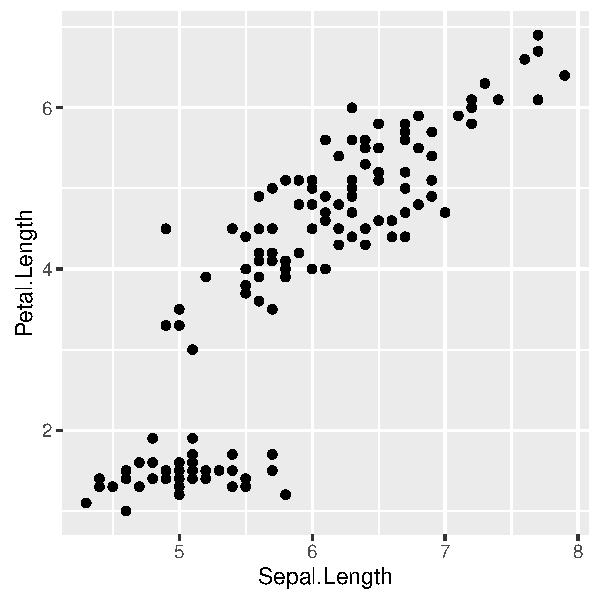
\includegraphics[width=\maxwidth]{figure/minimal-r17-1} 

}



\end{knitrout}
\subsection*{Adicionando color al gráfico}
\begin{knitrout}
\definecolor{shadecolor}{rgb}{0.969, 0.969, 0.969}\color{fgcolor}\begin{kframe}
\begin{alltt}
\hlkwd{ggplot}\hlstd{(iris,} \hlkwd{aes}\hlstd{(}\hlkwc{x} \hlstd{= Sepal.Length,} \hlkwc{y} \hlstd{= Petal.Length))} \hlopt{+}
  \hlkwd{geom_point}\hlstd{(}\hlkwd{aes}\hlstd{(}\hlkwc{color} \hlstd{= Species))}
\end{alltt}
\end{kframe}

{\centering 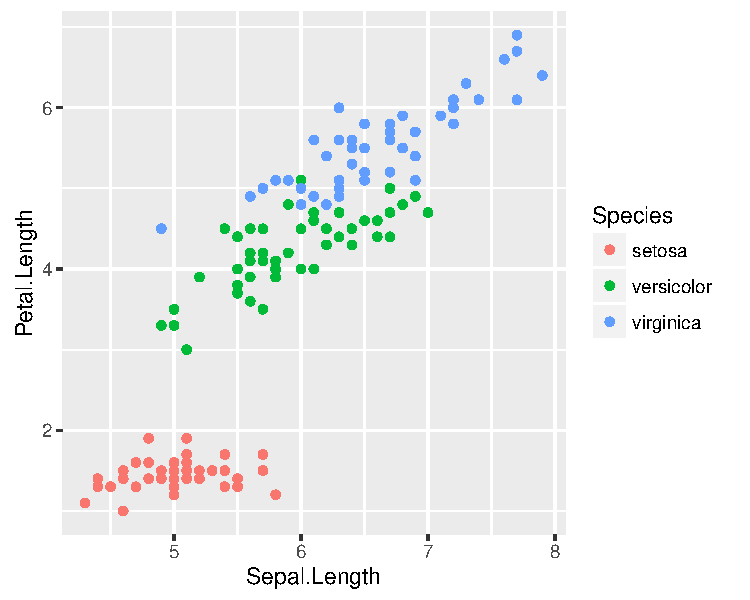
\includegraphics[width=\maxwidth]{figure/minimal-r18-1} 

}



\end{knitrout}


Realizado en la Universidad Distrital Francisco José de Caldas, Maestría en Ciencias de la Información y las Comunicaciones.\\

Se compilaron en total 18 chunks.
\end{document}
